\documentclass[11pt,a4paper]{article}
\usepackage[utf8]{inputenc}
\usepackage[T1]{fontenc}
\usepackage[spanish]{babel}
\usepackage{amsmath,amssymb}
\usepackage{graphicx}
\usepackage{booktabs}
\usepackage{float}
\usepackage[margin=2.5cm]{geometry}
\usepackage{hyperref}

\graphicspath{{figuras/}}   % guardar acá las figuras exportadas desde el notebook

\newcommand{\todo}[1]{\textbf{\textcolor{red}{[TODO: #1]}}}
\usepackage{xcolor}

\title{Trabajo Práctico 2\\[2pt]\large Compresión de imágenes sin pérdida mediante codificación de Huffman}
\author{Grupo XX \\ Integrante A, Integrante B}
\date{Inferencia y Estimación --- Primavera 2026}

\begin{document}
\maketitle

\begin{abstract}
Se comprimieron cinco imágenes en escala de grises con el código de Huffman, directamente píxel a píxel y sobre los residuos entre píxeles vecinos. Se midieron la entropía, la longitud media del código y la información mutua entre vecinos. Los residuos mejoraron fuertemente la compresión en cuatro de las cinco imágenes (entre $1{,}6\times$ y $2{,}8\times$, frente a $1{,}05\times$--$1{,}27\times$ píxel a píxel) pero empeoraron en la imagen con ruido granular (\texttt{img\_02}), donde la información mutua entre vecinos es casi nula.
\end{abstract}

%------------------------------------------------------------
\section{Introducción}
En este trabajo se estudia la compresión sin pérdida de imágenes en escala de grises con el código de Huffman, comparando dos representaciones: (i) cada intensidad de píxel como símbolo de la fuente, y (ii) la codificación diferencial mediante residuos entre píxeles vecinos. El objetivo es analizar cómo la dependencia entre píxeles vecinos, medida con la información mutua, afecta la eficiencia de la compresión.

\section{Metodología}
\subsection{Imágenes utilizadas}
Se trabajó con cinco imágenes: \texttt{img\_01} (camellos en el desierto, $568\times400$), \texttt{img\_02} (textura de arena, $612\times408$) e \texttt{img\_04} (partitura, $322\times224$), provistas por la cátedra, y dos imágenes agregadas por el grupo: \texttt{img\_03} (festejo del gol de Paredes al Vasco da Gama, $1256\times620$) e \texttt{img\_05} (Festejo icónico de Messi, $1605\times986$). Las dos últimas son bastante más grandes que las otras. Las imágenes originales son RGB y se convirtieron a escala de grises de 8 bits (intensidades $0$--$255$). Se muestran en la Figura~\ref{fig:imagenes} (ancho$\times$alto).

\begin{figure}[H]
\centering
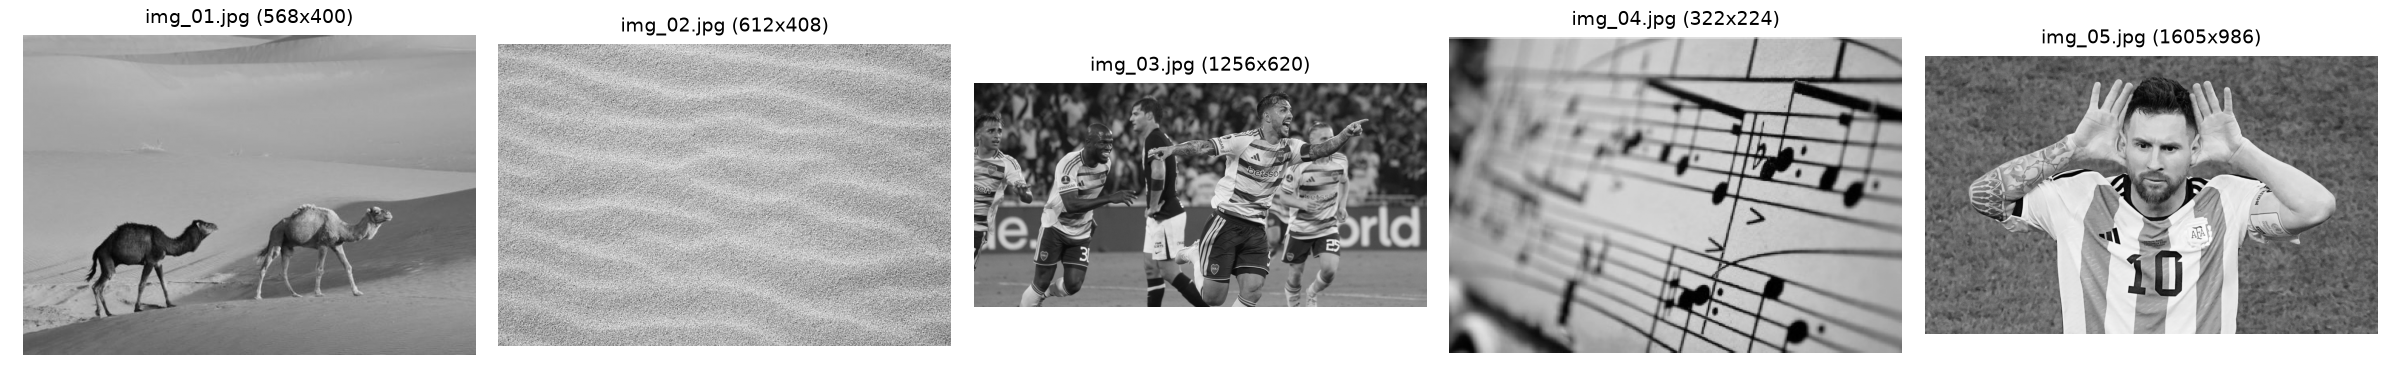
\includegraphics[width=\textwidth]{ej1_imagenes.png}
\caption{Imágenes utilizadas, en escala de grises.}
\label{fig:imagenes}
\end{figure}

\subsection{Estimación de probabilidades y entropía}
La masa de probabilidad se estima empíricamente a partir de las frecuencias relativas de cada valor en la imagen. La entropía es
\begin{equation}
H(X) = -\sum_x p(x)\log_2 p(x).
\end{equation}

\subsection{Codificación de Huffman}
Se utilizó la implementación provista por la cátedra para construir el código y decodificar. La longitud media teórica es $L=\sum_x p(x)\,l(x)$, que cumple $H(X)\le L<H(X)+1$. Los bits promedio reales se calculan como la longitud de la cadena codificada dividida por la cantidad de símbolos.

\subsection{Residuos}
Recorriendo cada fila de izquierda a derecha, el residuo es
\begin{equation}
y_{i,j}=x_{i,j}-x_{i,j-1},\qquad j=2,\dots,N,
\end{equation}
guardando el primer píxel de cada fila como condición inicial (8 bits por fila, incluidos en el costo total). No se calcula residuo entre el último píxel de una fila y el primero de la siguiente. La reconstrucción es $x_{i,j}=x_{i,j-1}+y_{i,j}$. Se verificó que la reconstrucción es exacta (sin pérdida) en todas las imágenes.

\subsection{Información mutua entre vecinos}
Para los pares $(X,X')=(x_{i,j-1},x_{i,j})$ usados en los residuos se estima
\begin{equation}
I(X;X')=H(X)+H(X')-H(X,X'),
\end{equation}
con $H(X,X')$ calculada a partir del histograma conjunto.

%------------------------------------------------------------
\section{Resultados}
\subsection{Ejercicio 1: codificación píxel a píxel}
\begin{figure}[H]
\centering
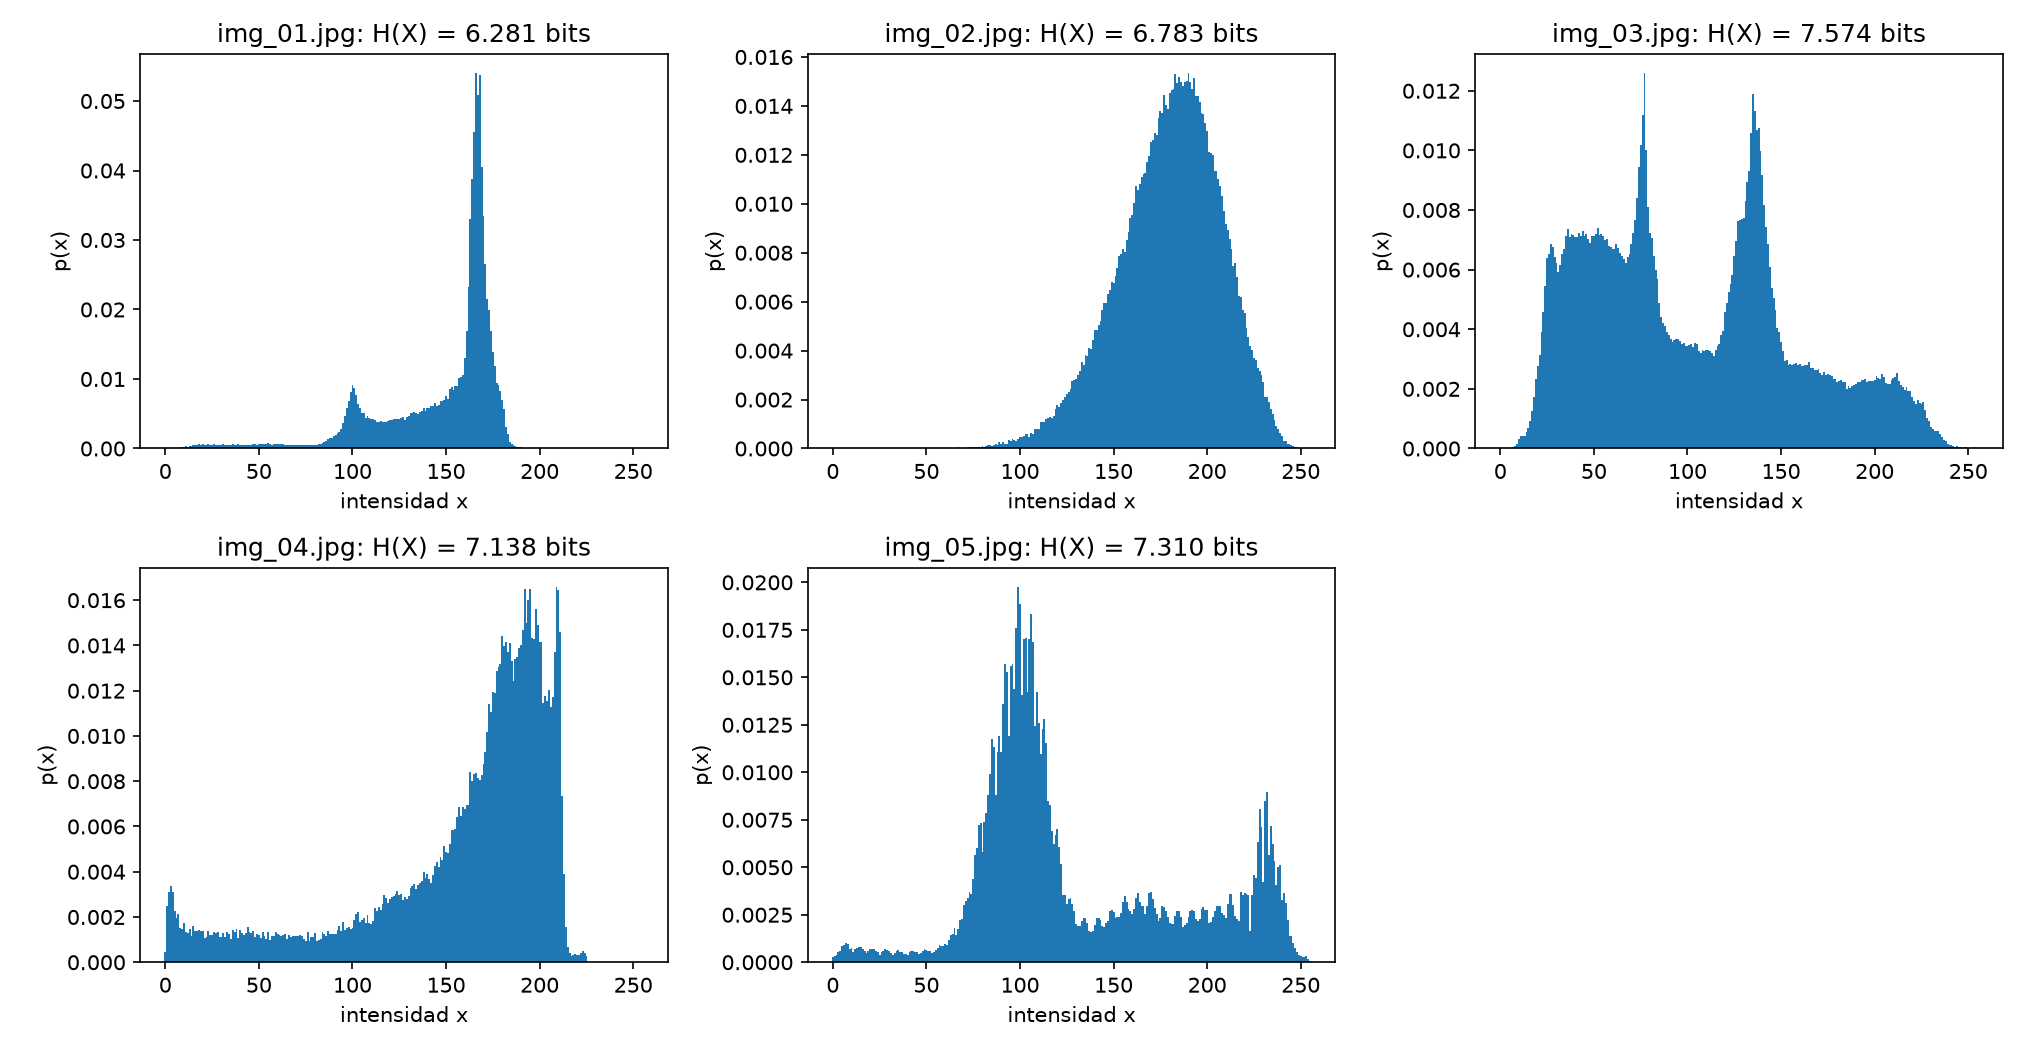
\includegraphics[width=\textwidth]{ej1_pmf.png}
\caption{Masa de probabilidad $p(x)$ de cada imagen, con su entropía $H(X)$.}
\label{fig:ej1}
\end{figure}

\begin{table}[H]
\centering
\begin{tabular}{lcccc}
\toprule
Imagen & $H(X)$ [bits] & $L$ [bits] & Bits prom.\ reales & Razón de compresión \\
\midrule
img\_01 & 6,281 & 6,310 & 6,310 & 1,268 \\
img\_02 & 6,783 & 6,809 & 6,809 & 1,175 \\
img\_03 & 7,574 & 7,600 & 7,600 & 1,053 \\
img\_04 & 7,138 & 7,165 & 7,165 & 1,117 \\
img\_05 & 7,310 & 7,338 & 7,338 & 1,090 \\
\bottomrule
\end{tabular}
\caption{Resultados del Ejercicio 1. Razón de compresión respecto de 8 bits/píxel.}
\end{table}
En las cinco imágenes se cumple $H(X)\le L<H(X)+1$, con $L$ solo entre $0{,}026$ y $0{,}029$ bits por encima de $H(X)$. Los bits promedio reales coinciden con $L$ porque el código se construye con la misma PMF con que se mide (no se cuenta el costo de almacenar la tabla del código). Las razones de compresión son modestas ($1{,}05$ a $1{,}27$), ya que el código solo aprovecha la forma del histograma.

\subsection{Ejercicio 2: codificación de residuos}
\begin{figure}[H]
\centering
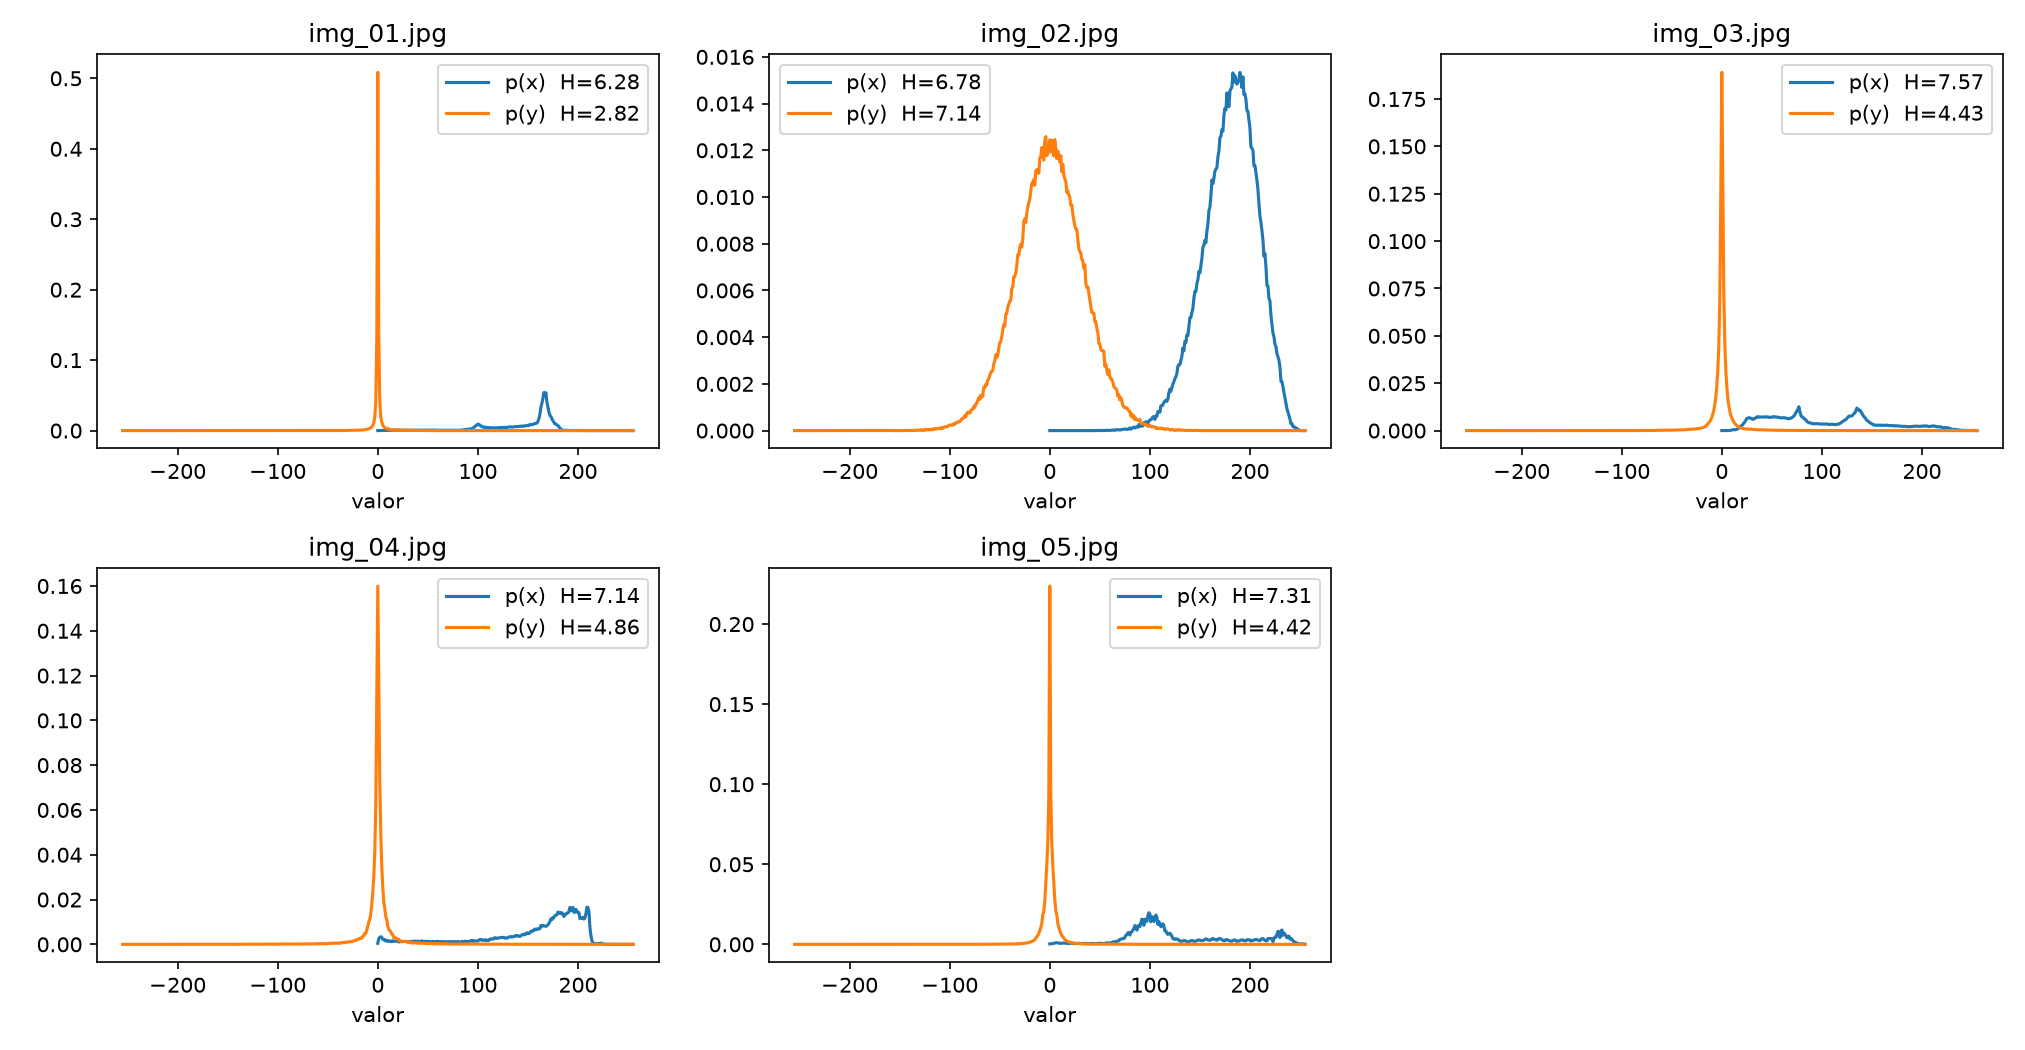
\includegraphics[width=\textwidth]{ej2_pmf.png}
\caption{$p(x)$ y $p(y)$ superpuestas para cada imagen, con sus entropías.}
\label{fig:ej2}
\end{figure}

\begin{table}[H]
\centering
\begin{tabular}{lccccc}
\toprule
Imagen & $H(X)$ & $H(Y)$ & $L_Y$ & Bits prom.\ reales (res.) & $I(X;X')$ \\
\midrule
img\_01 & 6,281 & 2,824 & 2,838 & 2,847 & 3,725 \\
img\_02 & 6,783 & 7,138 & 7,179 & 7,180 & 0,117 \\
img\_03 & 7,574 & 4,431 & 4,462 & 4,465 & 3,297 \\
img\_04 & 7,138 & 4,863 & 4,889 & 4,898 & 2,782 \\
img\_05 & 7,310 & 4,415 & 4,452 & 4,454 & 3,075 \\
\bottomrule
\end{tabular}
\caption{Resultados del Ejercicio 2 (en bits). La columna de bits promedio reales incluye el costo de los píxeles iniciales (8 bits por fila).}
\end{table}

Los bits promedio de los residuos solos coinciden con $L_Y$ ($2{,}838$; $7{,}179$; $4{,}462$; $4{,}889$ y $4{,}452$); los píxeles iniciales agregan menos de $0{,}01$ bit por píxel. Se verificó que decodificar y sumar los residuos reconstruye exactamente cada imagen.

\subsection{Ejercicio 4: compresor y descompresor \texttt{.tp2}}
Esta parte es opcional y no se desarrolla en el material de la cátedra: el diseño del formato \texttt{.tp2} y las herramientas para implementarlo (lectura de parámetros por terminal con \texttt{argparse}, empaquetado de bits en bytes con \texttt{numpy} y escritura binaria con \texttt{struct}) fueron investigados por el grupo por cuenta propia, a partir de la documentación de Python y de NumPy~\cite{pydocs}. Se implementaron dos programas de línea de comandos: \texttt{comprimir\_tp2.py imagen.jpg} genera \texttt{imagen.tp2}, y \texttt{descomprimir\_tp2.py imagen.tp2} reconstruye y muestra la imagen (con \texttt{-o} la guarda además en PNG). El formato binario (módulo \texttt{formato\_tp2.py}) guarda: un identificador, el alto y ancho, la tabla de Huffman de los residuos (símbolo, largo y código empaquetado), el primer píxel de cada fila (1 byte por fila) y los bits de los residuos empaquetados en bytes. Se verificó que la imagen descomprimida es idéntica a la imagen en escala de grises original, también en casos borde (imagen constante, de una fila o una columna, y de un solo píxel).

\begin{table}[H]
\centering
\begin{tabular}{lccc}
\toprule
Imagen & Tamaño \texttt{.tp2} [bytes] & Bits/píxel (archivo) & Razón vs.\ 8 bits \\
\midrule
img\_01 & 82\,197 & 2,894 & 2,76 \\
img\_02 & 225\,871 & 7,237 & 1,11 \\
img\_03 & 436\,578 & 4,485 & 1,78 \\
img\_04 & 45\,993 & 5,101 & 1,57 \\
img\_05 & 883\,294 & 4,465 & 1,79 \\
\bottomrule
\end{tabular}
\caption{Tamaño real de los archivos \texttt{.tp2}. Incluyen la tabla de Huffman, el encabezado y los píxeles iniciales.}
\end{table}

Los bits por píxel del archivo son algo mayores que los del Ejercicio 2 ($2{,}85$; $7{,}18$; $4{,}47$; $4{,}90$; $4{,}45$) por el costo de almacenar la tabla de Huffman y el encabezado, que antes no se contaba. Esa diferencia es de $0{,}05$ bit por píxel en \texttt{img\_01} y \texttt{img\_02}, de $0{,}2$ en la imagen más chica (\texttt{img\_04}) y de $0{,}02$ o menos en las dos más grandes (\texttt{img\_03} e \texttt{img\_05}): el costo fijo de la tabla pesa menos cuanto mayor es la imagen.

%------------------------------------------------------------
\section{Análisis}
\subsection{Diferencias de entropía entre imágenes}
La entropía mide cuán dispersa es $p(x)$. \texttt{img\_01} tiene la menor ($6{,}28$): grandes zonas de arena casi uniformes producen un pico marcado cerca de $x=167$. \texttt{img\_02} ($6{,}78$) tiene una campana ancha, de textura homogénea pero con grano. \texttt{img\_04} ($7{,}14$) combina fondo claro, notas y sombras oscuras, y reparte la probabilidad en casi todo el rango. \texttt{img\_05} ($7{,}31$) tiene un pico en tonos medios (el fondo, cerca de $x=100$) y otro en tonos claros (la camiseta), con mucha textura en el medio. \texttt{img\_03} tiene la mayor entropía ($7{,}57$): una escena compleja, con público y fondo oscuros, tonos medios y camisetas claras, cuyo histograma es multimodal y cubre casi todo el rango de intensidades. En resumen, la entropía depende de cuántos niveles de gris se usan y de cuán uniformemente.

\subsection{Significado de la información mutua}
$I(X;X')$ cuantifica cuánta incertidumbre sobre un píxel se elimina al conocer su vecino, es decir, cuán predecible es. Es alta en \texttt{img\_01} ($3{,}73$ bits), con zonas suaves; algo menor en las fotografías \texttt{img\_3} ($3{,}30$) e \texttt{img\_5} ($3{,}08$), que tienen grandes regiones suaves pero también bordes y texturas; menor en \texttt{img\_04} ($2{,}78$), con bordes marcados; y casi nula en \texttt{img\_02} ($0{,}12$), donde el grano es ruido prácticamente independiente entre vecinos. Se relaciona con el beneficio de los residuos: $H(X)-H(Y)$ vale $3{,}46$; $3{,}14$; $2{,}90$; $2{,}27$ y $-0{,}36$ respectivamente, en el mismo orden que $I(X;X')$. Además, siempre $I(X;X')\ge H(X)-H(Y)$: como $H(X|X')=H(Y|X')\le H(Y)$, vale $I(X;X')=H(X)-H(Y|X')\ge H(X)-H(Y)$. Es decir, la información mutua es una cota de cuánto puede ganarse al explotar a los vecinos, y los residuos simples (que no condicionan a $x_{i,j-1}$) capturan solo una parte.

\subsection{Píxel a píxel vs.\ residuos}
Los residuos reducen los bits por píxel de $6{,}31$ a $2{,}85$ en \texttt{img\_01} ($2{,}81\times$ de compresión frente a $1{,}27\times$), de $7{,}60$ a $4{,}47$ en \texttt{img\_03} ($1{,}79\times$ frente a $1{,}05\times$), de $7{,}34$ a $4{,}45$ en \texttt{img\_05} ($1{,}80\times$ frente a $1{,}09\times$) y de $7{,}17$ a $4{,}90$ en \texttt{img\_04} ($1{,}63\times$ frente a $1{,}12\times$). En todas, $p(y)$ es un pico muy concentrado en cero, porque los vecinos son similares, y esa estructura espacial es la redundancia que Huffman píxel a píxel no puede ver. Las dos fotografías (\texttt{img\_3} e \texttt{img\_5}) son las de mayor entropía píxel a píxel, o sea las que peor comprimen con ese método ($1{,}05\times$ y $1{,}09\times$), y sin embargo con residuos ganan cerca de $3$ bits por píxel: la entropía de $p(x)$ y la correlación entre vecinos son propiedades distintas. En \texttt{img\_02} ocurre lo contrario: los residuos empeoran ($7{,}18$ contra $6{,}81$ bits). Con ruido independiente de varianza $\sigma^2$, la diferencia de dos píxeles tiene varianza $2\sigma^2$, así que $p(y)$ es más ancha que $p(x)$ (Figura~\ref{fig:ej2}) y su entropía aumenta (en una gaussiana, $\tfrac12\log_2 2=0{,}5$ bit; se midieron $0{,}36$). Esta imagen casi no tiene redundancia entre vecinos que explotar. El costo de los píxeles iniciales es despreciable (menos de $0{,}01$ bit por píxel).

%------------------------------------------------------------
\section{Conclusiones}
Huffman es óptimo entre los códigos sin prefijo para una fuente de símbolos independientes: la longitud media quedó a menos de $0{,}03$ bits de la entropía en todos los casos. Pero solo explota la forma de la PMF, no la dependencia entre píxeles. La codificación por residuos modela esa dependencia y baja la entropía cuando hay correlación espacial: en las cuatro imágenes con $I(X;X')$ alta, los bits por píxel bajaron de $6{,}3$--$7{,}6$ a $2{,}8$--$4{,}9$ (razones de $1{,}6\times$ a $2{,}8\times$). En \texttt{img\_02}, con ruido granular y $I(X;X')\approx 0$, los residuos empeoraron ($7{,}18$ contra $6{,}81$). La información mutua entre vecinos es entonces un buen predictor de cuánto ayuda la codificación diferencial, y la entropía de $p(x)$ por sí sola no lo es (las fotografías de mayor entropía fueron de las que más ganaron). En los Ejercicios 1 y 2 no se contó el costo de almacenar la tabla de Huffman; el Ejercicio 4 sí lo incluye, y resultó despreciable en las imágenes grandes ($\le 0{,}02$ bit por píxel) pero no en las chicas ($0{,}2$ bit en \texttt{img\_04}).

\begin{thebibliography}{9}
\bibitem{huffman} D. A. Huffman, ``A Method for the Construction of Minimum-Redundancy Codes,'' \textit{Proceedings of the IRE}, vol.~40, no.~9, pp.~1098--1101, 1952.
\bibitem{shannon} C. E. Shannon, ``A Mathematical Theory of Communication,'' \textit{Bell System Technical Journal}, vol.~27, pp.~379--423, 623--656, 1948.
\bibitem{stathaki} T. Stathaki, \textit{Methods and Standards for Lossless Compression}, Digital Image Processing, Part 4: Image Compression, Imperial College.
\bibitem{pydocs} Documentación oficial de Python (módulos \texttt{argparse} y \texttt{struct}) y de NumPy (\texttt{packbits}, \texttt{unpackbits}), \url{https://docs.python.org/3/} y \url{https://numpy.org/doc/}.
\end{thebibliography}

\end{document}
